\documentclass[10pt]{article}

\usepackage{mathtools, amssymb, bm}
\usepackage{microtype}
\usepackage[utf8]{inputenc}
\usepackage[margin = 0.75in]{geometry}
\usepackage{booktabs}
\usepackage{graphicx}
\usepackage{xcolor}
\usepackage{tikzsymbols}
\usepackage[hidelinks]{hyperref}
\usepackage{titlesec}



% \titleformat{\section}{\normalsize\bfseries}{\thesection}{1em}{}
\titleformat{\section}{\large\bfseries}{\thesection}{1em}{}
\setcounter{secnumdepth}{0}

\definecolor{colabcol}{HTML}{960018}
\newcommand{\mycolab}[1]{\textcolor{colabcol}{\textsl{Collaborators:}} #1 \\ }
\newcommand{\mycolaba}[1]{\textcolor{colabcol}{\textsl{Collaborators:}} #1}

\title{
    {\Large Homework 4}
}
\author{
    {\normalsize Aiden Kenny}\\
    {\normalsize STAT GR5205: Linear Regression Models}\\
    {\normalsize Columbia University}
}
\date{\normalsize November 9, 2020}

\begin{document}

\maketitle

%' ============================================================================================================================================================
\section{Question 1} \noindent
\mycolab{None}
\begin{figure}[ht]
    \centering
    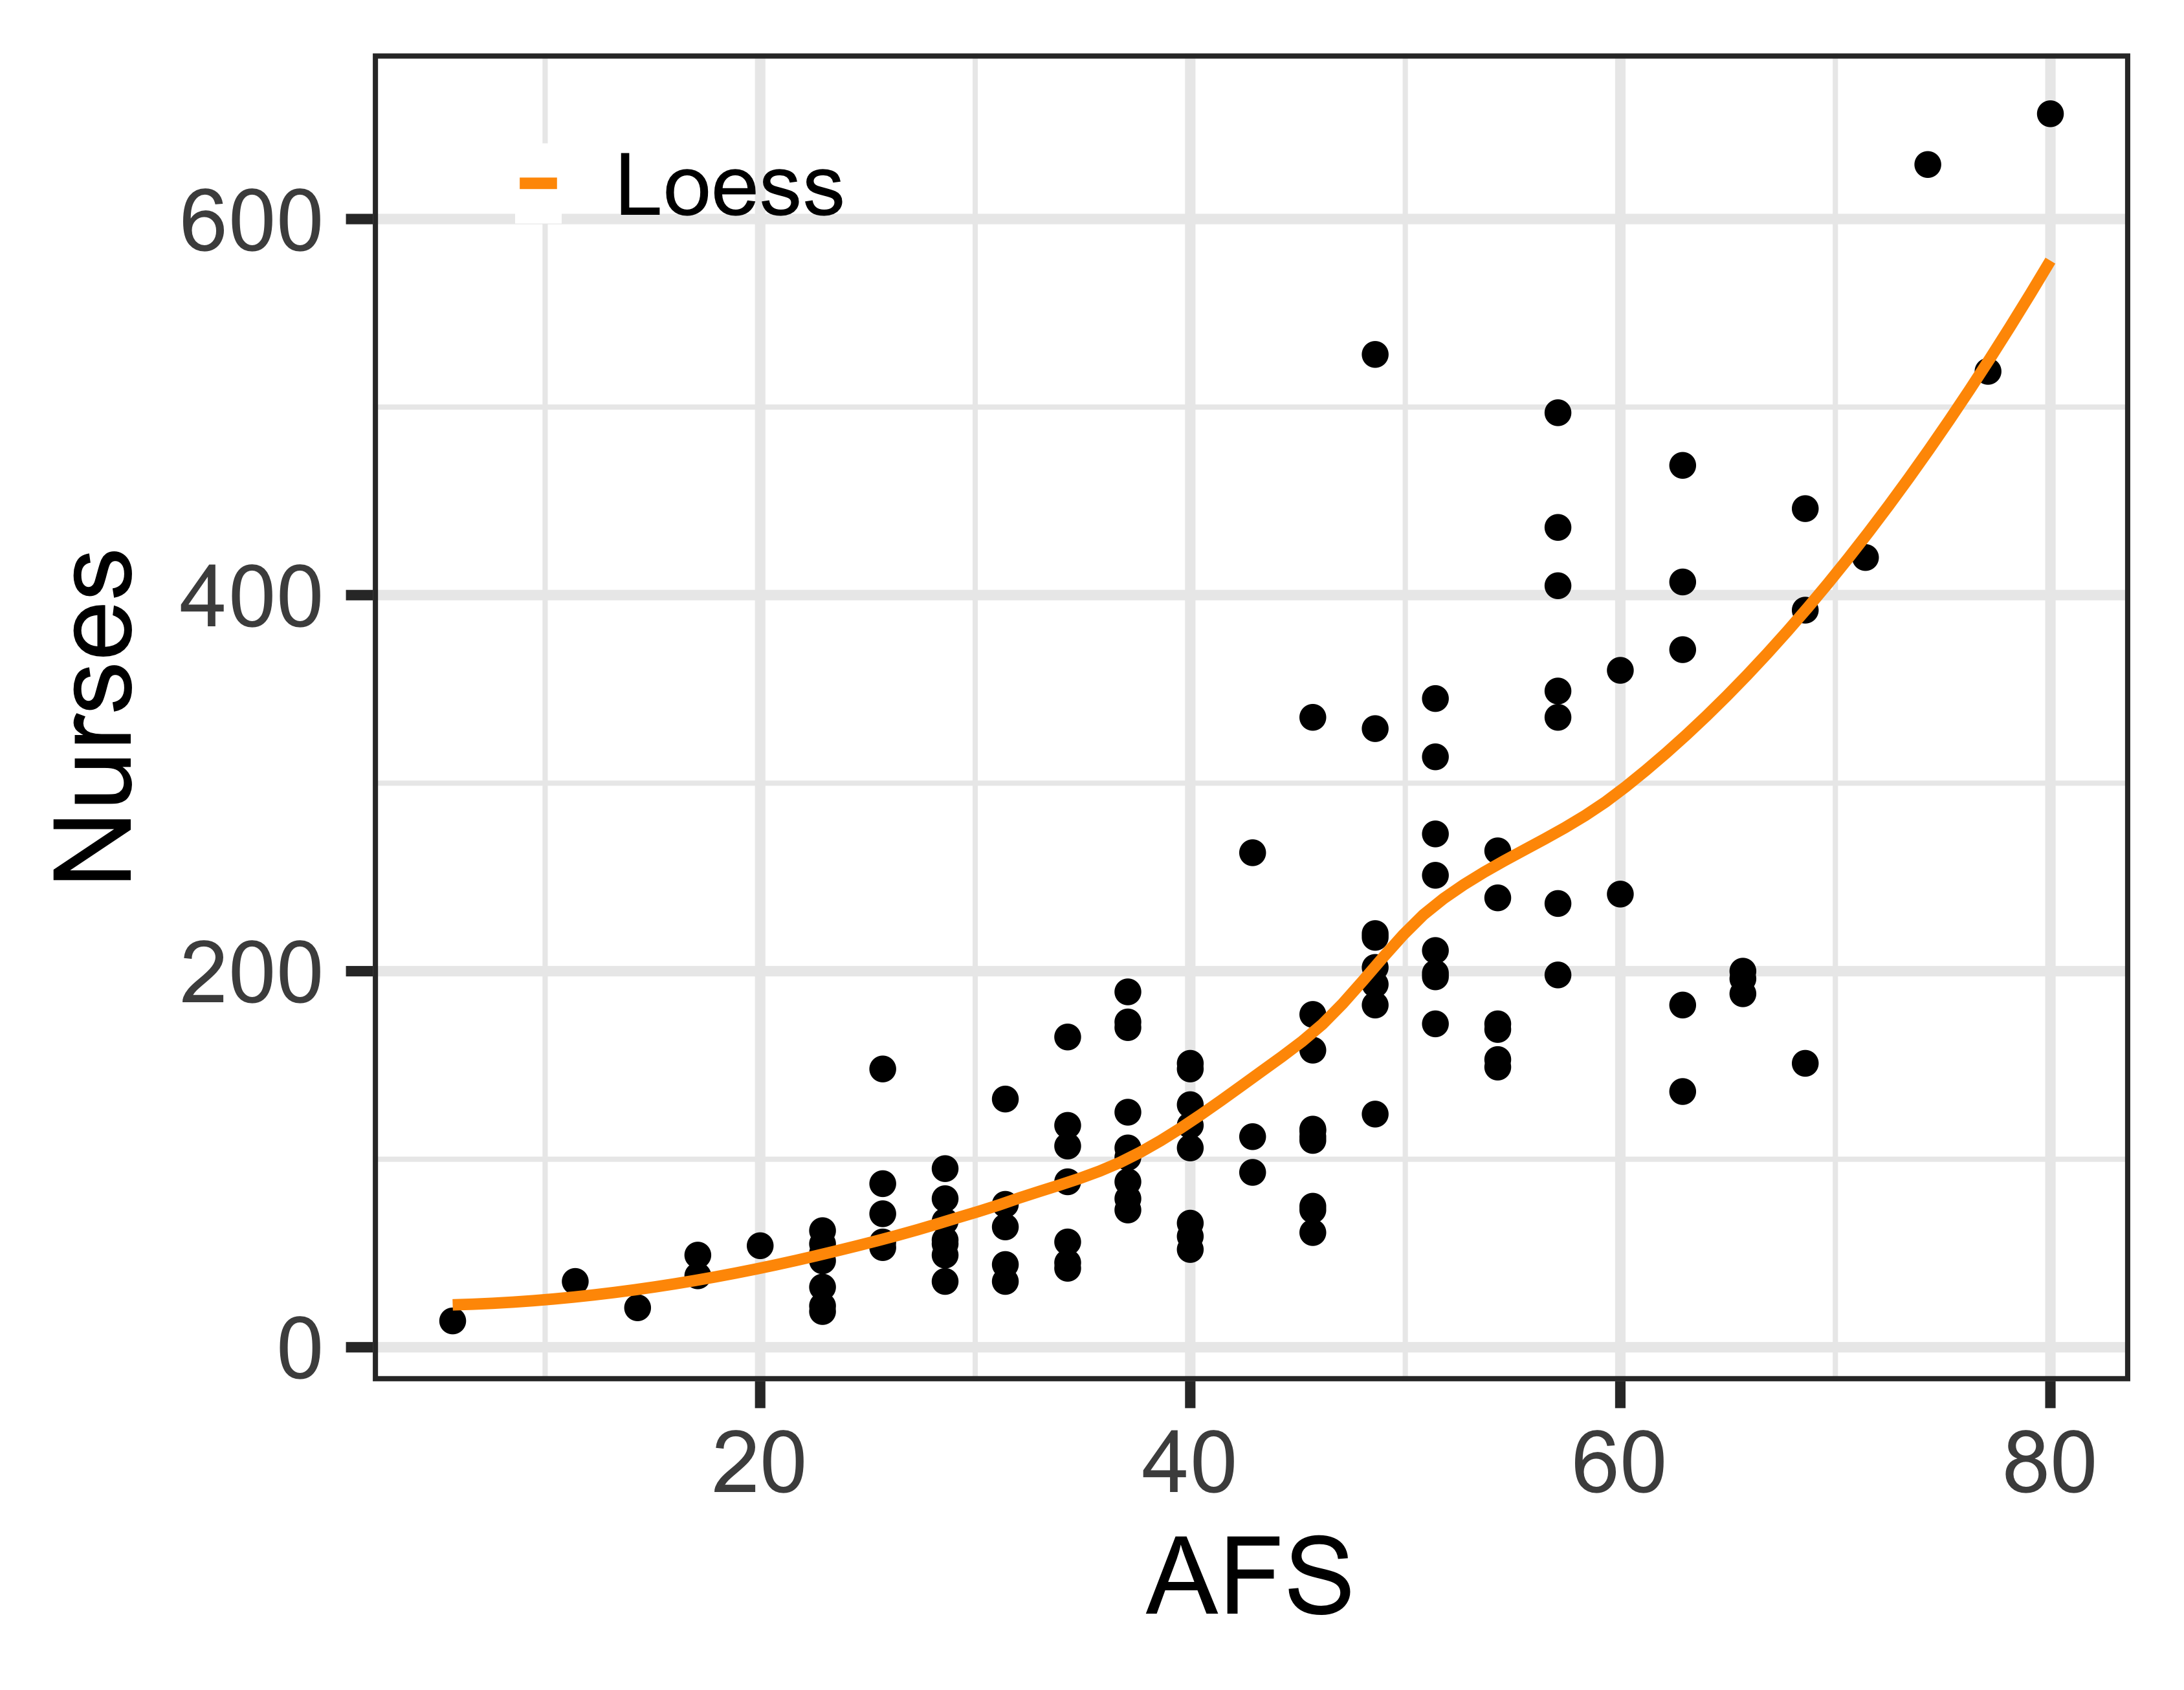
\includegraphics[width = 0.4\textwidth]{img/q01a-single.png}
    \quad
    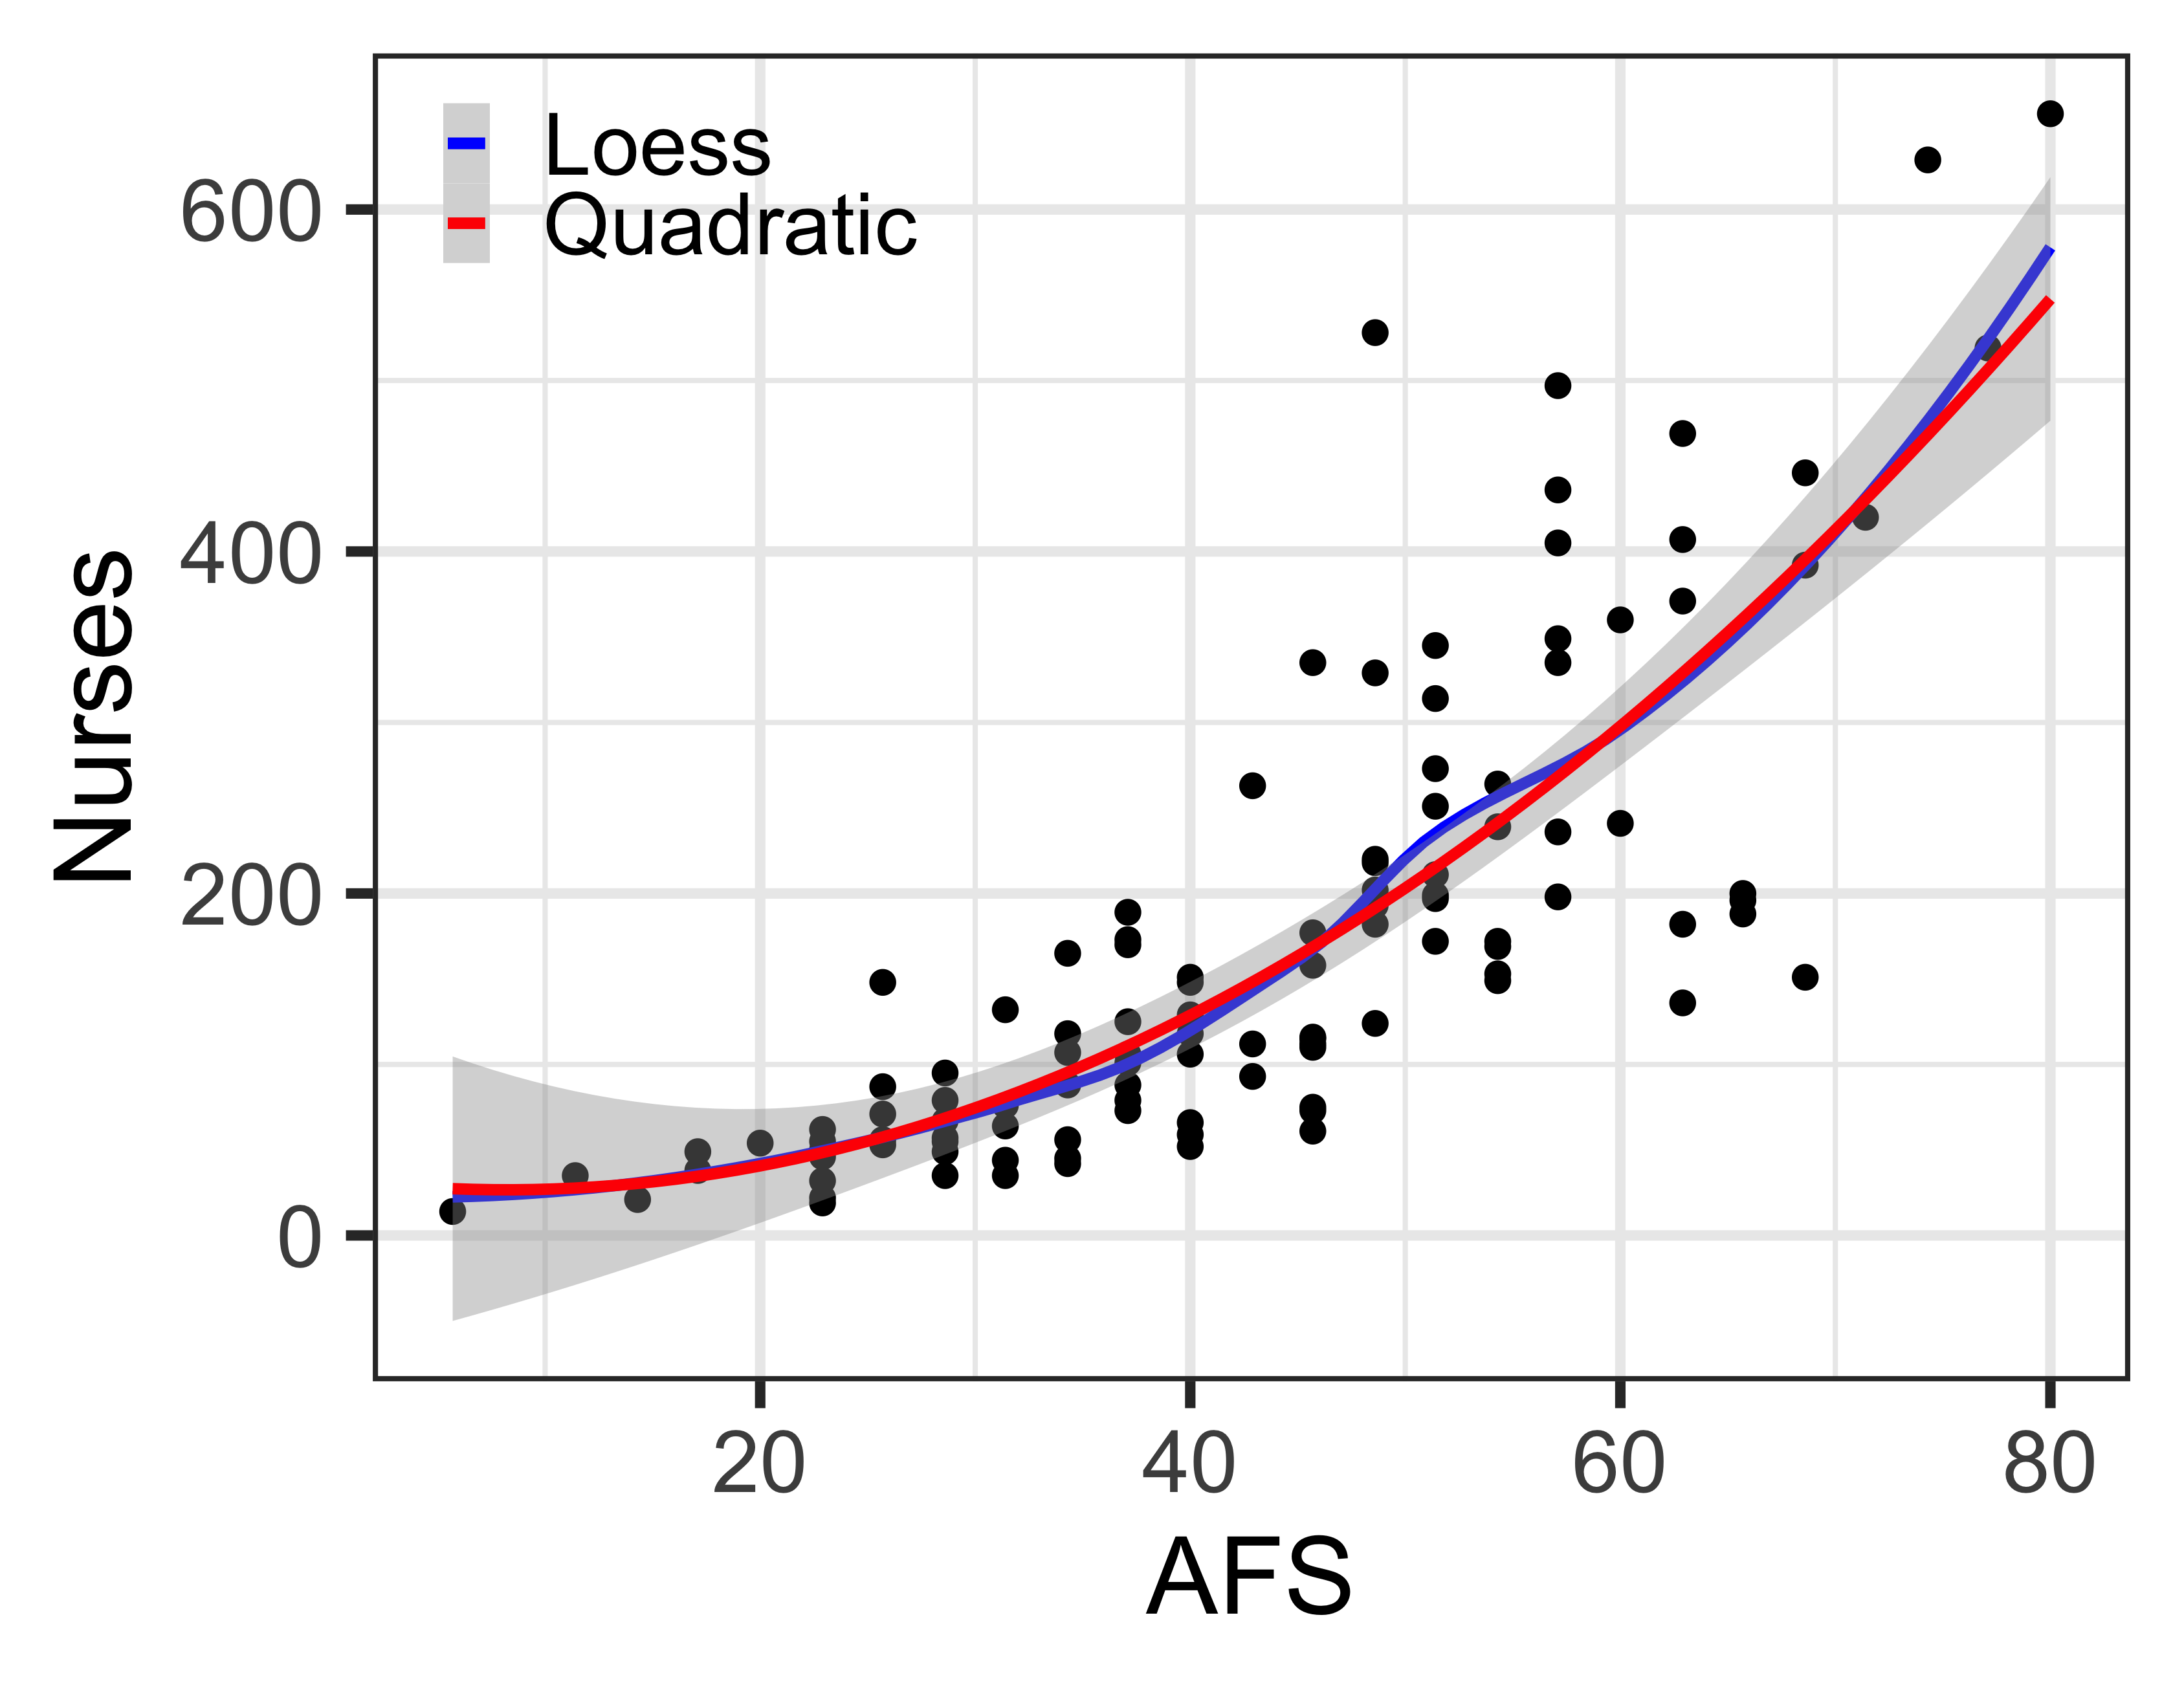
\includegraphics[width = 0.4\textwidth]{img/q01a-both.png}
    \caption{Overlaying a loess smoother and a quadratic polynomial to the scatterplot of AFS vs. Nurses.
    The left plot displays only the loess smoother, while the right plot displays both.}
    \label{fig-q01a}
\end{figure}
\begin{itemize}
    \item[(a)] The loess smoother is the blue line displayed in Figure \ref{fig-q01a}. For clarity, the left plot displays only the loess smoother. The loess 
    smoother indicates that a linear function does not seem plausible for this data, as the curve is too non-linear. 
    \item[(b)] The fitted quadratic model is given by \(\hat{Y} = 33.548 - 1.666 x + 0.101 x^2\), and can be see in the right panel of Figure \ref{fig-q01a}. 
    As we can see, the quadratic model almost perfectly overlays the loess smoother, further indicating that a linear relationship is not plausible. 
    \item[(c)] Given our model \(Y = \beta_0 + \beta_1 X + \beta_2 X^2 + \epsilon\), to determine if the quadratic term can be dropped from the model, we will
    test \(H_0 : \beta_2 = 0\) against \(H_a : \beta_2 \neq 0\). The \(p\)-value for this test is \(0.00032\), so for any reasonable significance level, we
    will reject \(H_0\). It seems that there is a non-negligible quadratic relationship. Interestingly, if one were to re-run the same test for \(\beta_0\) and 
    \(\beta_1\), the corresponding \(p\)-values would be \(0.515\) and \(0.495\), which would not give us grounds to reject either of those null hypotheses.
    That is, we could say the slope and linear term of this model are insignificant, but the quadratic term is not. 
    \item[(d)] 
\end{itemize}


%' ============================================================================================================================================================
\section{Question 2} \noindent



%' ============================================================================================================================================================
\section{Question 3} \noindent



%' ============================================================================================================================================================
\section{Question 4} \noindent
\mycolaba{None}
\begin{itemize}
    \item[(a)] For this question we will assume the matrix \(\mathbf{X}\) is \textsl{centered}, so that each predictor has mean zero. 
    In \(n\)-dimensional Euclidean vector space, for any \(\mathbf{v} \in \mathbb{R}^n\) we have \(\|\mathbf{v}\|^2 = \mathbf{v}^T\mathbf{v}\), 
    so the ridge regression loss function becomes 
    \begin{align*}
        Q(\bm{\beta}; \lambda) 
        = \| \mathbf{y} - \mathbf{X}\bm{\beta} \|^2 + \lambda \|\bm{\beta}\|^2
        = \mathbf{y}^T\mathbf{y} - 2 \bm{\beta}\mathbf{X}^T\mathbf{y} + \bm{\beta} \mathbf{X}^T \mathbf{X} \bm{\beta} + \lambda \bm{\beta}^T \bm{\beta}.
    \end{align*}
    Differentiating the loss function with respect to \(\bm{\beta}\) gives us 
    \begin{align*}
        \frac{\partial Q}{\partial \bm{\beta}}
        = -2 \mathbf{X}^T \mathbf{y} + 2 \mathbf{X}^T\mathbf{X}\bm{\beta} + 2 \lambda \bm{\beta}
        = -2 \mathbf{X}^T \mathbf{y} + 2 \big( \mathbf{X}^T\mathbf{X} + \lambda \mathbf{I} \big) \bm{\beta}
        \overset{\text{set}}{=} \mathbf{0},
    \end{align*}
    and finally solving for \(\bm{\beta}\) gives us 
    \(\hat{\bm{\beta}}_{\lambda} = \big( \mathbf{X}^T\mathbf{X} + \lambda \mathbf{I} \big)^{-1} \mathbf{X}^T\mathbf{y}\).
    \item[(b)] When \(\lambda = 0\) we have \(\hat{\bm{\beta}}_{\lambda = 0} = \big( \mathbf{X}^T\mathbf{X} \big)^{-1} \mathbf{X}^T\mathbf{y}\), the OLS 
    estimator. 
\end{itemize}

\end{document}